\documentclass[aspectratio=169,11pt]{beamer}

% ============================================================
%  Verdediging bachelorscriptie
%  Citatiestructuren in de Nederlandse rechtspraak
%  Vincent H.Z.R. Wiegman -- UvA
% ============================================================

\usepackage[utf8]{inputenc}
\usepackage[T1]{fontenc}
\usepackage{amsmath}
\usepackage{booktabs}
\usepackage{array}
\usepackage{tikz}
\usetikzlibrary{positioning,arrows.meta,calc,fit,backgrounds,shapes.geometric}

% ----------------------------- kleuren (UvA) -----------------
\definecolor{uvared}{HTML}{BC0031}
\definecolor{uvadark}{HTML}{1A1A1A}
\definecolor{uvagray}{HTML}{6E6E6E}
\definecolor{uvalight}{HTML}{F4F1EE}
\definecolor{uvablue}{HTML}{27548A}
\definecolor{uvagreen}{HTML}{2E7D5B}

% ----------------------------- thema -------------------------
\usetheme{default}
\usecolortheme{default}
\setbeamertemplate{navigation symbols}{}
\setbeamercolor{structure}{fg=uvared}
\setbeamercolor{normal text}{fg=uvadark}
\setbeamercolor{alerted text}{fg=uvared}
\setbeamercolor{frametitle}{fg=uvadark}
\setbeamercolor{title}{fg=uvadark}
\setbeamerfont{frametitle}{series=\bfseries}
\setbeamerfont{title}{series=\bfseries}
\setbeamertemplate{itemize items}[circle]
\setbeamercolor{itemize item}{fg=uvared}
\setbeamercolor{itemize subitem}{fg=uvagray}
\setbeamercolor{block title}{fg=white,bg=uvared}
\setbeamercolor{block body}{bg=uvalight}

% frametitle met rood streepje
\setbeamertemplate{frametitle}{%
  \vspace{0.6em}%
  {\color{uvared}\rule{0.5em}{0.9em}}\hspace{0.4em}%
  \insertframetitle\par
  \vspace{-0.3em}%
}

% footline
\setbeamertemplate{footline}{%
  \leavevmode%
  \hbox{%
  \begin{beamercolorbox}[wd=.38\paperwidth,ht=2.4ex,dp=1ex,leftskip=1em]{}%
    \tiny\color{uvagray}V.\,Wiegman%
  \end{beamercolorbox}%
  \begin{beamercolorbox}[wd=.50\paperwidth,ht=2.4ex,dp=1ex,center]{}%
    \tiny\color{uvagray}Citatiestructuren in de Nederlandse rechtspraak%
  \end{beamercolorbox}%
  \begin{beamercolorbox}[wd=.12\paperwidth,ht=2.4ex,dp=1ex,rightskip=1em]{}%
    \hfill\tiny\color{uvagray}\insertframenumber%
  \end{beamercolorbox}}%
  \vspace{0.2em}%
}


\newcommand{\rd}[1]{\textcolor{uvared}{#1}}
\newcommand{\gr}[1]{\textcolor{uvagray}{#1}}
\newcommand{\smallnote}[1]{{\footnotesize\color{uvagray}#1}}

\title{Citatiestructuren in de Nederlandse rechtspraak}
\subtitle{Een netwerkanalyse van macrostructuur, invloed en organisatie}
\author{Vincent H.Z.R. Wiegman}
\institute{Bachelor Informatiekunde \textperiodcentered{} Universiteit van Amsterdam}
\date{Verdediging \textperiodcentered{} Begeleider: Dr.\ M.J.\ Marx}

% ============================================================
\begin{document}

% ---------------------------------------------------------- 1
\begin{frame}[plain]
  \vspace{0.6cm}
  {\color{uvared}\rule{\textwidth}{1.4pt}}\\[0.5em]
  {\Large\bfseries Citatiestructuren in de Nederlandse rechtspraak}\\[0.3em]
  {\large Een netwerkanalyse van macrostructuur, invloed en organisatie}\\[1.0em]
  {\color{uvared}\rule{0.35\textwidth}{0.8pt}}\\[0.8em]
  \textbf{Vincent H.Z.R. Wiegman}\hspace{0.5em}\gr{(14661152)}\\[0.4em]
  Bachelor Informatiekunde \textperiodcentered{} Universiteit van Amsterdam\\[0.2em]
  \gr{Begeleider: Dr.\ M.J.\ Marx \textperiodcentered{} Semester 2, 2025--2026}
  \IfFileExists{uva_logo.png}{\hfill\includegraphics[height=1.1cm]{uva_logo}}{}
    \end{frame}

% ---------------------------------------------------------- 2
\begin{frame}{Rechtspraak als netwerk}
  \begin{columns}[T]
    \begin{column}{0.56\textwidth}
      \begin{itemize}
        \item Een uitspraak verwijst naar eerdere uitspraken om een beslissing te onderbouwen.
        \item Alle verwijzingen samen vormen een \rd{gericht citatienetwerk}: knoop = uitspraak, pijl = citatie.
        \item NL is een \emph{civil-law}-stelsel: \rd{geen \emph{stare decisis}}, toch citeren rechters eerdere uitspraken.
      \end{itemize}
      
    \end{column}
    \begin{column}{0.44\textwidth}
      \centering
      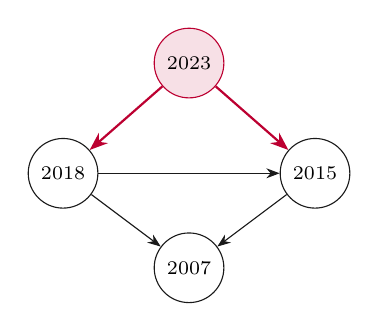
\begin{tikzpicture}[>=Stealth, every node/.style={font=\scriptsize}]
        \node[circle,draw=uvared,fill=uvared!12,minimum size=0.85cm] (a) at (0,0) {2023};
        \node[circle,draw=uvadark,fill=white,minimum size=0.7cm] (b) at (-1.6,-1.4) {2018};
        \node[circle,draw=uvadark,fill=white,minimum size=0.7cm] (c) at (1.6,-1.4) {2015};
        \node[circle,draw=uvadark,fill=white,minimum size=0.62cm] (d) at (0,-2.6) {2007};
        \draw[->,uvared,thick] (a) -- (b);
        \draw[->,uvared,thick] (a) -- (c);
        \draw[->,uvadark] (b) -- (d);
        \draw[->,uvadark] (c) -- (d);
        \draw[->,uvadark] (b) -- (c);
      \end{tikzpicture}\\[0.4em]
      \smallnote{Citaties wijzen in principe \emph{terug in de tijd}.}
    \end{column}
  \end{columns}
\end{frame}

% ---------------------------------------------------------- 3
\begin{frame}{Onderzoeksvraag}
  \begin{block}{Hoofdvraag}
    Welke \rd{structurele eigenschappen} vertoont het Nederlandse jurisprudentie\-citatienetwerk van Rechtspraak.nl, en hoe is \rd{juridische invloed} verdeeld over uitspraken, rechtsgebieden en rechterlijke instanties?
  \end{block}
  \vspace{0.3em}
  \footnotesize
  \begin{enumerate}
    \item Macrostructuur: componenten, bow-tie, k-core.
    \item Verdeling van invloed: in-degree, PageRank, HITS-authority; is er een power-law?
    \item Overeenstemming tussen de maten.
    \item Communities (Leiden) vs.\ de juridische rechtsgebieden.
    \item Citatieflow tussen instanties en assortativity in de hi\"erarchie.
  \end{enumerate}
\end{frame}

% ---------------------------------------------------------- 5
\begin{frame}{De vijf deelvragen}
  \footnotesize
  \renewcommand{\arraystretch}{1.35}
  \begin{tabular}{@{}p{0.5cm} p{4.3cm} p{8.0cm}@{}}
    \toprule
    & \textbf{Vraag} & \textbf{Kernbevinding} \\
    \midrule
    DV1 & Macrostructuur & Samenhangend maar \rd{vrijwel acyclisch}: grootste WCC 73,6\%, grootste SCC slechts 26 knopen. \\
    DV2 & Verdeling van invloed & \rd{Extreem geconcentreerd}; zware staart, maar power-law niet aantoonbaar boven log-normaal. \\
    DV3 & Overeenstemming maten & In-degree $\approx$ PageRank (Spearman 0,880), HITS-authority wijkt af. \\
    DV4 & Communities vs.\ rechtsgebieden & Communities vrijwel zuiver, maar fijner dan de hoofdgebieden. \\
    DV5 & Citaties tussen instanties & Assortativity \rd{licht positief} ($r=0{,}105$), tegen de verwachting in. \\
    \bottomrule
  \end{tabular}
  \vspace{0.6em}

  \centering
  {\color{uvared}\rule{0.6\textwidth}{0.6pt}}\\[0.3em]
  Vandaag licht ik er \textbf{twee} uit: \rd{HITS-authority} (DV2/3) en de \rd{positieve assortativity} (DV5)
\end{frame}

% ============================================================
\begin{frame}[plain]
  \centering
  \vspace{1.4cm}
  {\color{uvared}\rule{0.5\textwidth}{1.2pt}}\\[0.7em]
  {\Large\bfseries Dataset}\\[0.4em]
  {\large De ``terug-in-de-tijd''-citaties}\\[0.7em]
  {\color{uvared}\rule{0.5\textwidth}{1.2pt}}
\end{frame}


% ---------------------------------------------------------- 4
\begin{frame}{Data: van LIDO naar de jurisprudentie-subgraaf}
  \footnotesize
  \begin{columns}[T]
    \begin{column}{0.6\textwidth}
      \begin{table}
        \centering\renewcommand{\arraystretch}{1.15}
        \begin{tabular}{@{}lrr@{}}
          \toprule
          Stap & Edges & Knopen \\
          \midrule
          Ruwe export (LIDO) & 7.355.861 & --- \\
          Hele netwerk & 6.917.225 & 1.628.457 \\
          Alleen jurisprudentie $\to$ jurisprudentie & 1.353.673 & 674.590 \\
          Na zelfverwijzingen \& deduplicatie & 1.353.664 & 674.589 \\
          \rd{Na temporeel onmogelijke ($-130.206$)} & \rd{1.223.458} & \rd{674.589} \\
          \bottomrule
        \end{tabular}
      \end{table}
    \end{column}
    \begin{column}{0.38\textwidth}
      \begin{block}{Eindnetwerk}
        \centering
        \textbf{674.589} knopen\\
        \textbf{1.223.458} citaties\\
        dichtheid $2{,}69\times10^{-6}$
      \end{block}
    \end{column}
  \end{columns}
  \vspace{0.5em}
  \smallnote{Verwijzingen automatisch uit documentteksten afgeleid: alleen \emph{bestaan} van een citatie, niet de functie (instemmend / afwijzend).}
\end{frame}


% ---------------------------------------------------------- 15
\begin{frame}{Temporeel onmogelijke citaties: waarschijnlijk een detectie-artefact}
  \footnotesize
  \begin{columns}[T]
    \begin{column}{0.56\textwidth}
      \begin{itemize}
        \item Een citatie loopt per definitie van \rd{later} naar \rd{eerder}.
        \item Toch: \rd{130.206 edges (9,62\%)} waarbij de citerende uitspraak \emph{ouder} is dan de geciteerde.
        \item Sterk geconcentreerd op enkele recente \rd{EHRM}-knopen (2022--2024).
        \item De grootste: \emph{Nam a.o.\ v.\ Russia} (EHRM, 26 okt.\ 2023) met 21.160 inkomende citaties, \rd{86\% van v\'o\'or} de uitspraakdatum; oudste uit \textbf{1882}.
        \item Een \rd{verzamelpunt} voor EVRM-verwijzingen, geen echte citaties.
      \end{itemize}
    \end{column}
    \begin{column}{0.44\textwidth}
      \centering
      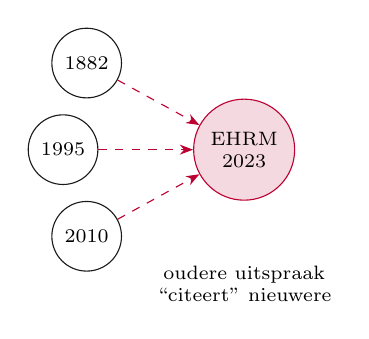
\begin{tikzpicture}[>=Stealth, every node/.style={font=\scriptsize}]
        \node[circle,draw=uvared,fill=uvared!15,minimum size=1.1cm,align=center] (ehrm) at (0,0) {EHRM\\2023};
        \node[circle,draw=uvadark,fill=white,minimum size=0.55cm] (o1) at (-2.0,1.1) {1882};
        \node[circle,draw=uvadark,fill=white,minimum size=0.55cm] (o2) at (-2.3,0.0) {1995};
        \node[circle,draw=uvadark,fill=white,minimum size=0.55cm] (o3) at (-2.0,-1.1) {2010};
        \draw[->,uvared,dashed] (o1) -- (ehrm);
        \draw[->,uvared,dashed] (o2) -- (ehrm);
        \draw[->,uvared,dashed] (o3) -- (ehrm);
        \node[align=center,font=\scriptsize] at (0,-1.7) {oudere uitspraak\\ ``citeert'' nieuwere};
      \end{tikzpicture}
    \end{column}
  \end{columns}
  \vspace{0.3em}
  \begin{block}{Interpretatie}
    Deze edges zijn verwijderd, daarna wordt HITS-authority pas betekenisvol (Haviltex bovenaan). Het patroon wijst op \rd{bugs in de referentie-detectie}, niet op echte verwijzingen.
  \end{block}
\end{frame}



\begin{frame}[plain]
  \centering
  \vspace{1.4cm}
  {\color{uvared}\rule{0.5\textwidth}{1.2pt}}\\[0.7em]
  {\Large\bfseries Verdieping 1}\\[0.4em]
  {\large HITS-authority en de kern van standaardarresten}\\[0.7em]
  {\color{uvared}\rule{0.5\textwidth}{1.2pt}}
\end{frame}

% ---------------------------------------------------------- 7
\begin{frame}{Drie invloedmaten, drie heel verschillende verdelingen}
  \footnotesize
  \begin{table}
    \centering\renewcommand{\arraystretch}{1.2}
    \begin{tabular}{@{}lcccc@{}}
      \toprule
      Maat & Gini & top-1\% & top-10\% & \\
      \midrule
      In-degree & 0,772 & 36,0\% & 67,9\% & \gr{breed} \\
      MARC-in-degree \smallnote{(van Opijnen)} & 0,586 & 6,8\% & 39,3\% & \gr{log-schaal} \\
      PageRank & 0,447 & 19,1\% & 40,0\% & \gr{breed} \\
      \rd{HITS-authority} & \rd{0,994} & \rd{93,0\%} & \rd{99,9\%} & \rd{extreem} \\
      \bottomrule
    \end{tabular}
  \end{table}
  \vspace{0.4em}
  \begin{itemize}
    \item In-degree en PageRank meten \rd{brede} invloed en lijken sterk op elkaar.
    \item HITS-authority is veel schever: de top-1\% bevat 93\% van alle authority.
    \item[$\Rightarrow$] \textbf{Waarom legt HITS-authority bijna al het gewicht op zo'n kleine groep?}
  \end{itemize}
\end{frame}

% ---------------------------------------------------------- 8
\begin{frame}{De top-authority is \'e\'en standaardarrest}
  \footnotesize
  \begin{columns}[T]
    \begin{column}{0.54\textwidth}
      \begin{table}
        \centering\renewcommand{\arraystretch}{1.15}
        \begin{tabular}{@{}llr@{}}
          \toprule
          Uitspraak & Authority & In-degree \\
          \midrule
          \rd{HR:1981:AG4158} \smallnote{(Haviltex)} & \rd{0,2211} & \rd{5.365} \\
          HR:2004:AO1427 & 0,0313 & 901 \\
          HR:2007:AZ3178 & 0,0127 & 312 \\
          HR:2022:853 & 0,0106 & 2.745 \\
          CE:ECHR:2023:\ldots & 0,0083 & 3.024 \\
          \bottomrule
        \end{tabular}
      \end{table}
      \vspace{0.3em}
      \begin{itemize}
        \item Haviltex: $\approx 7\times$ zo hoog als nummer twee.
        \item Top-100 authorities: \rd{92 van de Hoge Raad}.
        \item Hubs = vrijwel alle \rd{PHR-conclusies} die naar die arresten verwijzen.
      \end{itemize}
    \end{column}
    \begin{column}{0.46\textwidth}
      \centering
      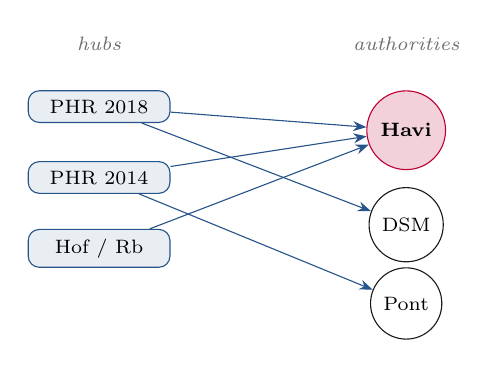
\begin{tikzpicture}[>=Stealth, every node/.style={font=\scriptsize}, node distance=0.35cm]
        % hubs
        \node[draw=uvablue,fill=uvablue!10,rounded corners,minimum width=1.8cm] (h1) at (-2.2,1.0) {PHR 2018};
        \node[draw=uvablue,fill=uvablue!10,rounded corners,minimum width=1.8cm] (h2) at (-2.2,0.1) {PHR 2014};
        \node[draw=uvablue,fill=uvablue!10,rounded corners,minimum width=1.8cm] (h3) at (-2.2,-0.8) {Hof / Rb};
        % authorities
        \node[circle,draw=uvared,fill=uvared!18,minimum size=1.0cm] (a1) at (1.7,0.7) {\textbf{Havi}};
        \node[circle,draw=uvadark,fill=white,minimum size=0.7cm] (a2) at (1.7,-0.5) {DSM};
        \node[circle,draw=uvadark,fill=white,minimum size=0.62cm] (a3) at (1.7,-1.5) {Pont};
        \foreach \h in {h1,h2,h3}{
          \draw[->,uvablue] (\h) -- (a1);
        }
        \draw[->,uvablue] (h1) -- (a2);
        \draw[->,uvablue] (h2) -- (a3);
        \node[font=\scriptsize\itshape,uvagray] at (-2.2,1.8) {hubs};
        \node[font=\scriptsize\itshape,uvagray] at (1.7,1.8) {authorities};
      \end{tikzpicture}\\[0.3em]
      \smallnote{Goede hubs verwijzen naar goede authorities, en omgekeerd.}
    \end{column}
  \end{columns}
\end{frame}

% ---------------------------------------------------------- 9
\begin{frame}{Het mechanisme: het \emph{tightly-knit community}-effect}
  \begin{itemize}
    \item HITS-authority is de \rd{principale eigenvector van $A^{\!\top}A$} (de co-citatiematrix).
    \item PHR-conclusies citeren steeds \rd{dezelfde kern} van standaardarresten samen $\Rightarrow$ die arresten zijn onderling sterk \emph{co-geciteerd}.
    \item De eigenvector legt daardoor bijna al het gewicht op die ene dichte kern, en \rd{bijna niets} op de rest, ook niet op uitspraken met hoge in-degree (Lempel \& Moran, 2001).
  \end{itemize}
  \vspace{0.3em}
  \begin{block}{Conclusie}
    Authority meet \rd{geen brede invloed}, maar een \rd{positioneel kenmerk}: het lidmaatschap van een kleine, dicht co-geciteerde kern $\Rightarrow$ in-degree en PageRank blijven primair.
  \end{block}
\end{frame}


% ============================================================
\begin{frame}[plain]
  \centering
  \vspace{1.4cm}
  {\color{uvared}\rule{0.5\textwidth}{1.2pt}}\\[0.7em]
  {\Large\bfseries Verdieping 2}\\[0.4em]
  {\large Assortativity: waarom \emph{positief} en niet negatief?}\\[0.7em]
  {\color{uvared}\rule{0.5\textwidth}{1.2pt}}
\end{frame}

% ---------------------------------------------------------- 11
\begin{frame}{De verwachting: negatieve assortativity}
  \begin{columns}[T]
    \begin{column}{0.55\textwidth}
      \begin{itemize}
        \item Het stelsel is hi\"erarchisch: Rechtbank $\to$ Gerechtshof $\to$ Hoge Raad.
        \item Lagere instanties zoeken precedent bij \rd{hogere} instanties.
        \item Newman-assortativity $r$ op instantietype: \\[0.2em]
          \quad $r<0$ = ``citaties tussen typen'' (hi\"erarchie)\\
          \quad $r>0$ = ``soort citeert soort'' (homofilie)
        \item Verwachting voor een cassatie-stelsel: \rd{$r<0$}.
      \end{itemize}
    \end{column}
    \begin{column}{0.45\textwidth}
      \centering
      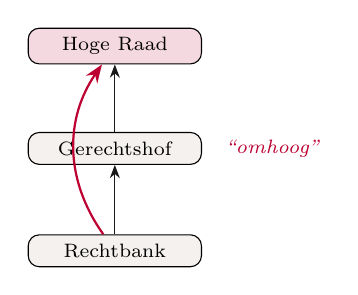
\begin{tikzpicture}[>=Stealth, every node/.style={font=\scriptsize}]
        \node[draw,rounded corners,fill=uvared!15,minimum width=2.2cm] (hr) at (0,2.0) {Hoge Raad};
        \node[draw,rounded corners,fill=uvalight,minimum width=2.2cm] (hof) at (0,0.7) {Gerechtshof};
        \node[draw,rounded corners,fill=uvalight,minimum width=2.2cm] (rb) at (0,-0.6) {Rechtbank};
        \draw[->,uvared,thick] (rb) to[bend left=35] (hr);
        \draw[->,uvadark] (rb) -- (hof);
        \draw[->,uvadark] (hof) -- (hr);
        \node[font=\scriptsize\itshape,uvared] at (2.0,0.7) {``omhoog''};
      \end{tikzpicture}
    \end{column}
  \end{columns}
\end{frame}

% ---------------------------------------------------------- 12
\begin{frame}{Het resultaat: $r=+0{,}105$ en toch stroomt invloed omhoog}
  \footnotesize
  \begin{columns}[T]
    \begin{column}{0.5\textwidth}
      \begin{table}
        \centering\renewcommand{\arraystretch}{1.25}
        \begin{tabular}{@{}lrr@{}}
          \toprule
          Richting & Citaties & \% \\
          \midrule
          Lager $\to$ hoger & 377.951 & 35,4\% \\
          Hoger $\to$ lager & 153.957 & 14,4\% \\
          Zelfde niveau & 536.933 & 50,2\% \\
          \bottomrule
        \end{tabular}
      \end{table}
      \vspace{0.4em}
      \begin{itemize}
        \item Opwaartse flow \rd{is} aanwezig: $\approx 2{,}5:1$.
        \item Toch is $r$ \emph{positief}. Hoe kan dat?
      \end{itemize}
    \end{column}
    \begin{column}{0.5\textwidth}
      \begin{block}{Observatie}
        Een sterke ``lager $\to$ hoger''-stroom zou $r$ \rd{negatief} moeten maken. De helft van alle citaties blijft echter \emph{op hetzelfde niveau}, vooral citaties \emph{binnen het eigen instantietype}.
      \end{block}
    \end{column}
  \end{columns}
\end{frame}

% ---------------------------------------------------------- 13
\begin{frame}{Twee mechanismen verhogen de co\"effici\"ent}
  \footnotesize
  \begin{columns}[T]
    \begin{column}{0.55\textwidth}
      \textbf{1. Zelfverwijzende bestuursrechters}\\
      RvS, CRvB en CBb citeren vooral zichzelf:
      \begin{table}
        \centering\renewcommand{\arraystretch}{1.1}
        \begin{tabular}{@{}lr@{}}
          \toprule
          Instantie & \% binnen eigen type \\
          \midrule
          Raad van State & 67,4\% \\
          Centrale Raad van Beroep & 63,5\% \\
          College van Beroep bedr.\ & 80,5\% \\
          \midrule
          Rechtbank / Gerechtshof & 16,0\% / 14,2\% \\
          \bottomrule
        \end{tabular}
      \end{table}
      \textbf{2. Volume van Rb en Hof}\\
      Hun \emph{kleine} interne aandeel levert door hun \emph{grote aantal} toch veel interne verbindingen op.
    \end{column}
    \begin{column}{0.45\textwidth}
      \centering
      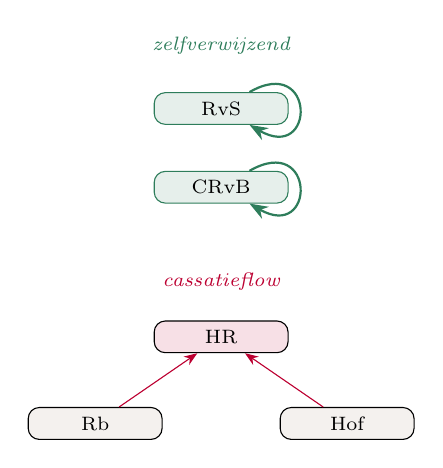
\begin{tikzpicture}[>=Stealth, every node/.style={font=\scriptsize}]
        % zelfverwijzend cluster
        \node[draw=uvagreen,fill=uvagreen!12,rounded corners,minimum width=1.7cm] (rvs) at (0,1.6) {RvS};
        \node[draw=uvagreen,fill=uvagreen!12,rounded corners,minimum width=1.7cm] (crvb) at (0,0.6) {CRvB};
        \draw[->,uvagreen,thick] (rvs) to[out=30,in=-30,looseness=6] (rvs);
        \draw[->,uvagreen,thick] (crvb) to[out=30,in=-30,looseness=6] (crvb);
        \node[uvagreen,font=\scriptsize\itshape] at (0,2.4) {zelfverwijzend};
        % cassatieflow
        \node[draw,rounded corners,fill=uvared!12,minimum width=1.7cm] (hr) at (0,-1.3) {HR};
        \node[draw,rounded corners,fill=uvalight,minimum width=1.7cm] (rb) at (-1.6,-2.4) {Rb};
        \node[draw,rounded corners,fill=uvalight,minimum width=1.7cm] (hof) at (1.6,-2.4) {Hof};
        \draw[->,uvared] (rb) -- (hr);
        \draw[->,uvared] (hof) -- (hr);
        \node[uvared,font=\scriptsize\itshape] at (0,-0.6) {cassatieflow};
      \end{tikzpicture}
    \end{column}
  \end{columns}
  \vspace{0.2em}
  \smallnote{De zelfverwijzing + het volume compenseren de cassatieflow $\Rightarrow$ een kleine \emph{positieve} co\"effici\"ent in plaats van de verwachte negatieve.}
\end{frame}

% ---------------------------------------------------------- 16
\begin{frame}{Conclusie}
  \begin{itemize}
    \item Het netwerk is \rd{samenhangend maar vrijwel acyclisch}: een tijdgeordend citatienetwerk, geen bow-tie zoals het WWW.
    \item Invloed is \rd{extreem ongelijk} verdeeld: de keuze van maat bepaalt vooral \emph{hoe sterk} de concentratie is, minder \emph{welke} uitspraken bovenaan staan.
    \item In-degree en PageRank zijn uitwisselbaar voor brede invloed, HITS-authority is een positionele maat.
    \item Drie organiserende principes: \rd{tijdsordening}, \rd{specialisatie naar rechtsgebied}, \rd{institutionele hi\"erarchie}.
  \end{itemize}
  \vspace{0.5em}
  \centering
  {\color{uvared}\rule{0.6\textwidth}{0.6pt}}\\[0.4em]
  \textbf{Bedankt \textemdash{} vragen?}
\end{frame}




\begin{frame}{Macrostructuur (DV1)}
  \footnotesize
  \begin{columns}[T]
    \begin{column}{0.5\textwidth}
      \begin{itemize}
        \item WCC: 93.587 componenten; grootste \rd{496.679 (73,6\%)}.
        \item SCC: 612.286; grootste slechts \rd{26 knopen (0,004\%)} , \ WWW $\approx 28\%$.
        \item Grootste SCC: lokale cluster RBZWB (25) + GHSHE (1).
        \item Bow-tie: TENDRILS\_OUT 25,1\%, OTHER 43,1\%, TUBES 0.
        \item k-core max $k=19$ (109 knopen), \rd{gedomineerd door rechtbanken}, niet door HR/RvS.
      \end{itemize}
    \end{column}
  \end{columns}
\end{frame}


\begin{frame}{Power-law of log-normaal (DV2)}
  \footnotesize
  Procedure van Clauset et al.\ (2009): maximum-likelihood-fit + likelihood-ratio-test ($R>0$ = power-law beter, $R<0$ = alternatief beter).
  \begin{table}
    \centering\renewcommand{\arraystretch}{1.15}
    \begin{tabular}{@{}llccc@{}}
      \toprule
      Maat & vs.\ log-normaal & $\alpha$ & $R$ & $p$ \\
      \midrule
      In-degree & lognormal & 2,47 & $-0{,}33$ & 0,742 \\
      PageRank & lognormal & 2,37 & $-1{,}42$ & 0,157 \\
      HITS-authority & lognormal & 2,27 & $+0{,}12$ & 0,902 \\
      \bottomrule
    \end{tabular}
  \end{table}
  \begin{itemize}
    \item Exponent $\alpha\approx 2$ (gebruikelijk voor citatienetwerken), \emph{maar} geen enkele maat verslaat log-normaal significant.
    \item Zware staart: ja. Power-law als verklarend model: \rd{niet aan te nemen} ( Broido \& Clauset, 2019).
  \end{itemize}
\end{frame}

% --- backup: overeenstemming maten
\begin{frame}{Overeenstemming tussen maten (DV3)}
  \footnotesize
  \begin{table}
    \centering\renewcommand{\arraystretch}{1.2}
    \begin{tabular}{@{}lcc@{}}
      \toprule
      Paar & Spearman $\rho$ & Kendall $\tau$ \\
      \midrule
      In-degree vs.\ PageRank & \rd{0,880} & 0,759 \\
      In-degree vs.\ HITS-authority & 0,639 & 0,537 \\
      PageRank vs.\ HITS-authority & 0,388 & 0,293 \\
      \bottomrule
    \end{tabular}
  \end{table}
  \begin{itemize}
    \item Top-10 Jaccard in-degree/PageRank $= 0{,}54$ (7 van de 10 gedeeld).
    \item MARC = monotone transformatie van in-degree $\Rightarrow$ \emph{identieke} rangschikking.
    \item Leeftijdseffect zwak ($\rho=0{,}191$): PageRank plaatst oude, sterk geciteerde uitspraken een fractie lager.
  \end{itemize}
\end{frame}


\begin{frame}{Communities vs.\ rechtsgebieden (DV4)}
  \footnotesize
  \begin{itemize}
    \item Leiden op de WCC: $Q\approx 0{,}86$; \rd{272 communities} (seed met hoogste $Q$).
    \item Dekking labels: 91\% (Bestuur 337k, Civiel 140k, Straf 135k).
    \item \rd{Lage ARI (0,079)} + \rd{hoge homogeniteit (0,723)}: communities intern zuiver, maar elk rechtsgebied is over veel communities verdeeld.
    \item Specifiek niveau (31 gebieden): NMI stijgt naar 0,380 $\Rightarrow$ communities $\approx$ \emph{deelgebieden}, niet de vier hoofdgebieden.
    \item Community 13 (zuiverheid 0,72): mengt straf/civiel/bestuur, stabiel over seeds $\Rightarrow$ een onderwerp dat meerdere rechtsgebieden raakt.
  \end{itemize}
\end{frame}



\end{document}